\documentclass{standalone}
\usepackage{amsmath}
\usepackage[dvipsnames]{xcolor}
\usepackage{tikz} 
\usetikzlibrary{arrows, decorations.markings,decorations.pathreplacing,angles,quotes}
\usepackage{microtype}
\usepackage{fourier}

\definecolor{py_blue}{rgb}{0.12156862745098039, 0.4666666666666667, 0.7058823529411765}
\definecolor{py_orange}{rgb}{1.0, 0.4980392156862745, 0.054901960784313725}
\definecolor{py_green}{rgb}{0.17254901960784313, 0.6274509803921569, 0.17254901960784313}
\definecolor{py_red}{rgb}{0.8392156862745098, 0.15294117647058825, 0.1568627450980392}
\definecolor{py_purple}{rgb}{0.5803921568627451, 0.403921568627451, 0.7411764705882353}

\begin{document}

\begin{tikzpicture}
	\node[anchor=south west,inner sep=0] (Bild) at (0,0) {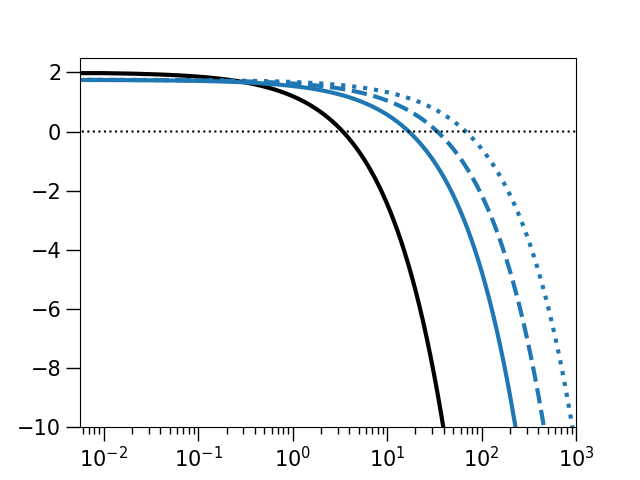
\includegraphics[scale=0.39]{ampicillin_blank}};
   		\begin{scope}[x=(Bild.south east),y=(Bild.north west)]
   			\node (Bild2) at ([xshift=2.75cm]Bild.east) {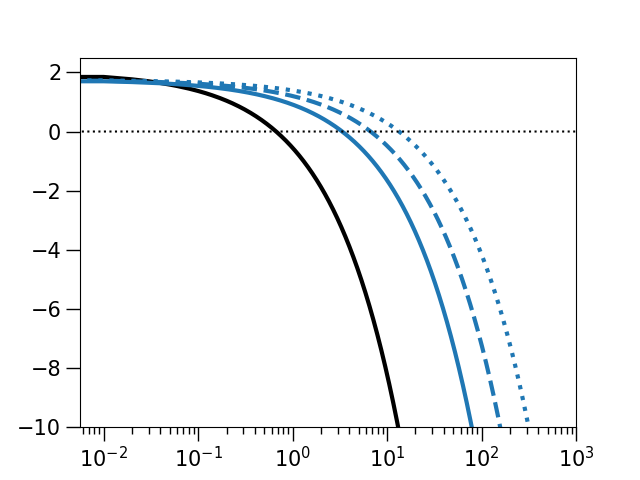
\includegraphics[scale=0.39]{tetracycline_blank}};
   			%\node (B3) at ([xshift=2.75cm]Bild2.east) {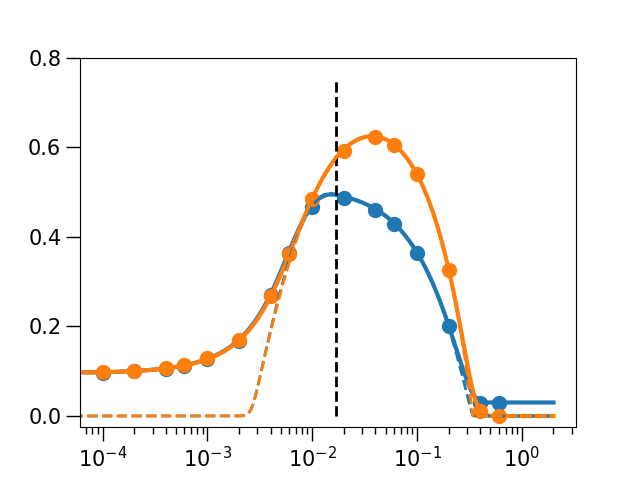
\includegraphics[scale=.39]{birth_high_blank}};
        	
			\node (B4) at ([yshift=-2.75cm]Bild.south) {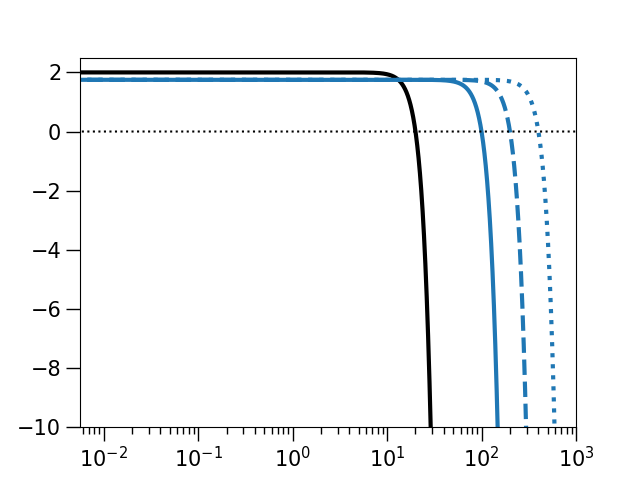
\includegraphics[scale=.39]{hypoSteep_blank}};
			\node (B5) at ([xshift=2.75cm]B4.east) {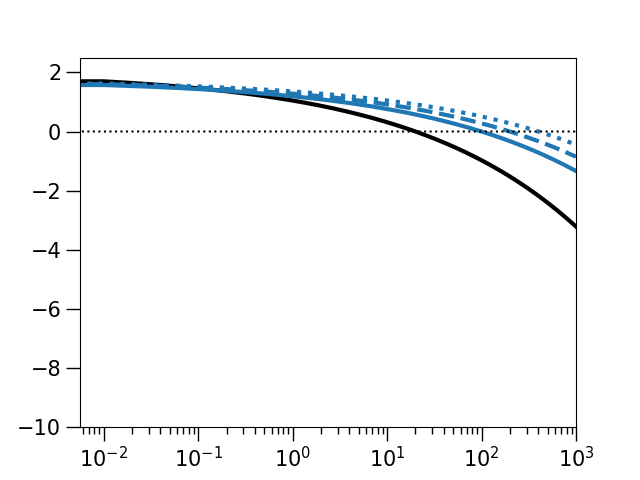
\includegraphics[scale=0.39]{hypoFlat_blank}};
   			%\node (B6) at ([xshift=2.75cm]B5.east) {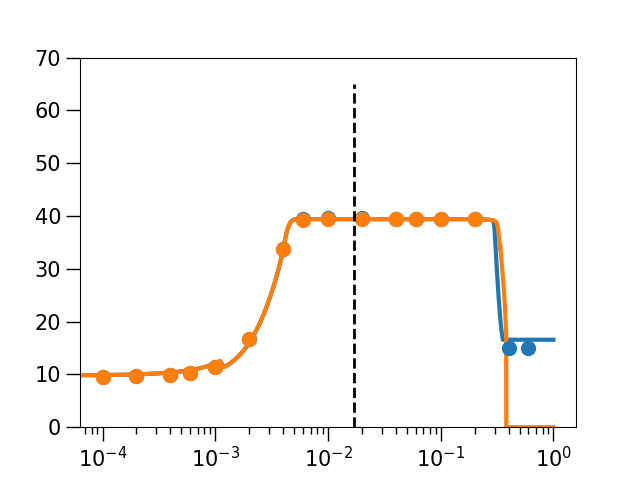
\includegraphics[scale=.39]{death_high_blank}};        	
        	
        	\node at ([xshift=-3cm,yshift=-.2cm]B5.south) {\Large antibiotic concentration $c$};
        	\node[rotate=90] at ([xshift=-.4cm,yshift=-2.55cm]Bild.west) {\Large pathogen growth rate $(\beta_k-\delta_k-\alpha_k(c)$)};
        	%\node at ([yshift=-.2cm]Bild.north) {\Large $\text{mic}_R = 5\times \text{mic}_S$};
        	%\node at ([yshift=-.3cm]Bild2.north) {\Large $\text{mic}_R = 10\times \text{mic}_S$};
        	%\node at ([yshift=-.3cm]B3.north) {\Large $\text{mic}_R = 20\times \text{mic}_S$};
        	
        	\node at ([yshift=-.1cm]Bild.north) {ampicillin};
        	\node at ([yshift=-.2cm]Bild2.north) {tetracycline};
        	\node at ([yshift=-.2cm]B4.north) {hypothetical steep};
        	\node at ([yshift=-.2cm]B5.north) {hypothetical flat};
        	       	
			\draw[thick,color=black] (1.14,-0.6) -- node[right=5pt] {\scriptsize \color{black} sensitive MIC, $\text{mic}_S$} (1.19,-0.6);        	
			\draw[thick,color=py_blue] (1.14,-0.68) -- node[right=5pt] {\scriptsize \color{black} weak resistance, $\text{mic}_R=5\times\text{mic}_S$} (1.19,-0.68);     
			\draw[thick,color=py_blue,dashed] (1.14,-0.76) -- node[right=5pt] {\scriptsize \color{black} intermediate res., $\text{mic}_R=10\times\text{mic}_S$} (1.19,-0.76);  
			\draw[thick,color=py_blue,dotted] (1.14,-0.84) -- node[right=5pt] {\scriptsize \color{black} strong resistance, $\text{mic}_R=20\times\text{mic}_S$} (1.19,-0.84);    
			
			%\node at (0.475,0.7) {\scriptsize msw};  
 			
    	\end{scope}
\end{tikzpicture}

\end{document}